\documentclass[11pt]{article}
\usepackage{fancyhdr}
\usepackage{enumerate}
\usepackage{array}
\usepackage{graphicx}
\newcommand{\tab}{\hspace*{2em}}
\pdfpagewidth 8.5in
\pdfpageheight 11in
\usepackage[margin=1.4in]{geometry}
\pagestyle{fancy}
\headheight 35pt

\rhead{Spatial ENSO Index Report}
%\chead{Spatial ENSO Index}
\lhead{Matthew Le}
\rfoot{7/26/2012}
\cfoot{\thepage}
\lfoot{Summer 2012}

\begin{document}
\section{Randomized Cross Validation}
This section shows the results from the cross validation experiment that was performed.  For each index we have the ``original'' correlation (non-randomized), where one year gets left out of the training set, and the rest of the years are used for multivariate regression.  We take the beta values from the regression function and try to predict with the one year that gets left out.  At the end, we correlate the predictions with their actual values.  The histogram shows 1000 trials of performing this cross validation, but where the target values get randomized each trial
\subsection{NINO 3.4 Index}
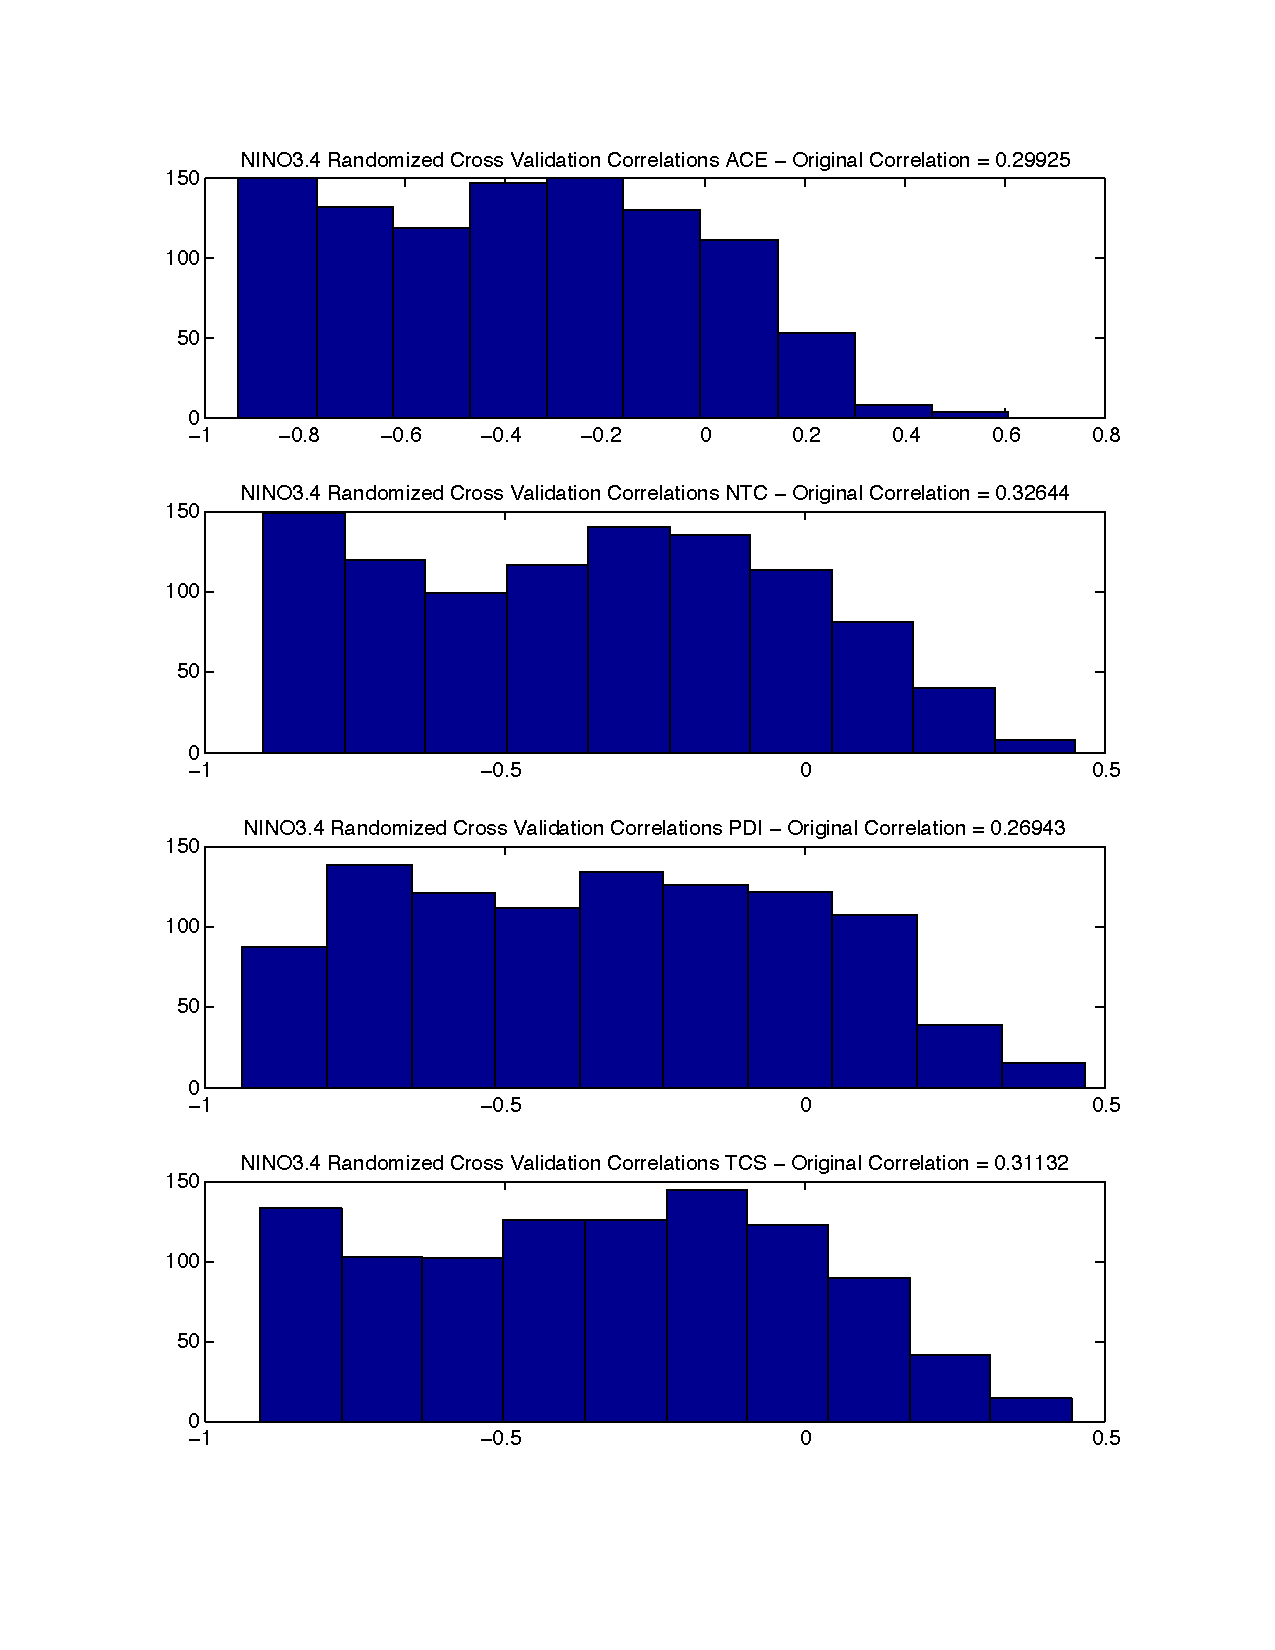
\includegraphics [ scale=0.62 ]{images/randomizedCrossValidationNINO.pdf}
\newpage
\subsection{Spatial OLR Index}
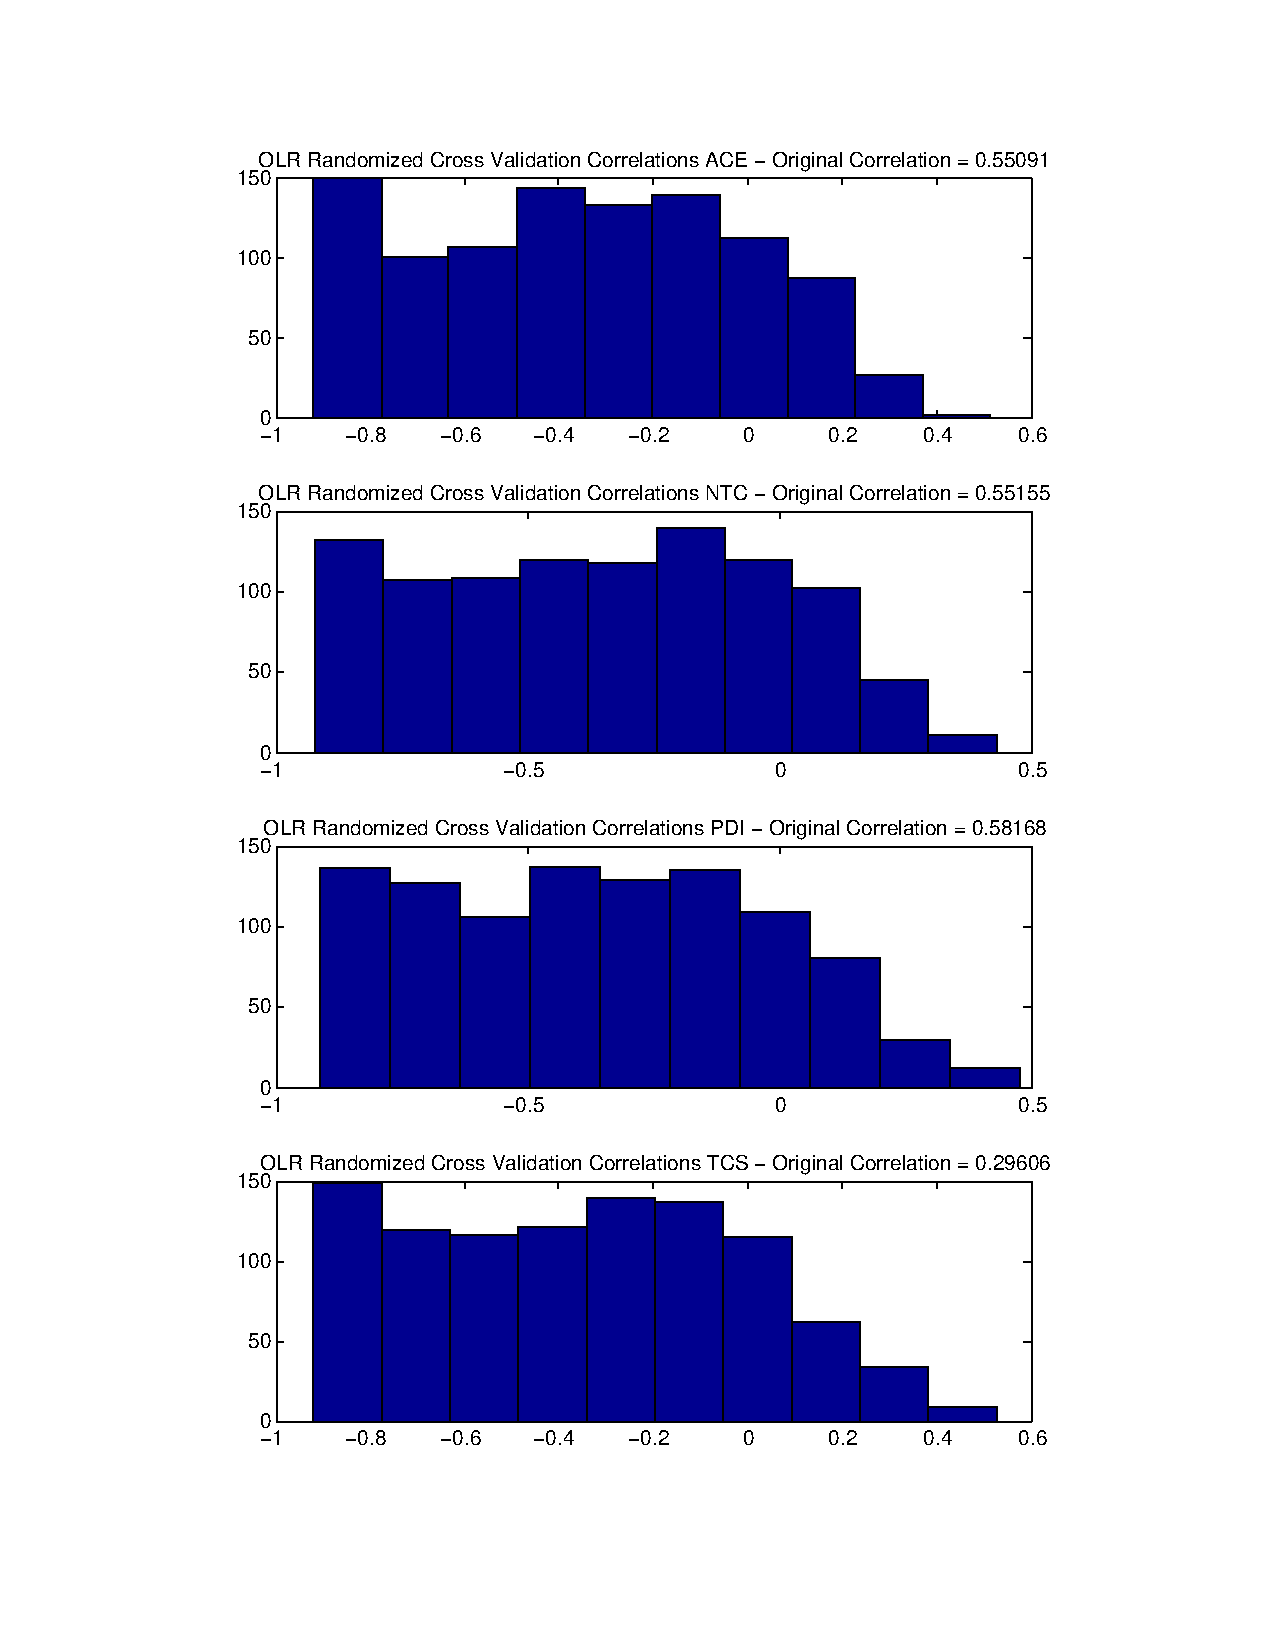
\includegraphics[ scale=0.7]{images/randomizedCrossValidationOLR.pdf}
\newpage
\subsection{Spatial SST Index}
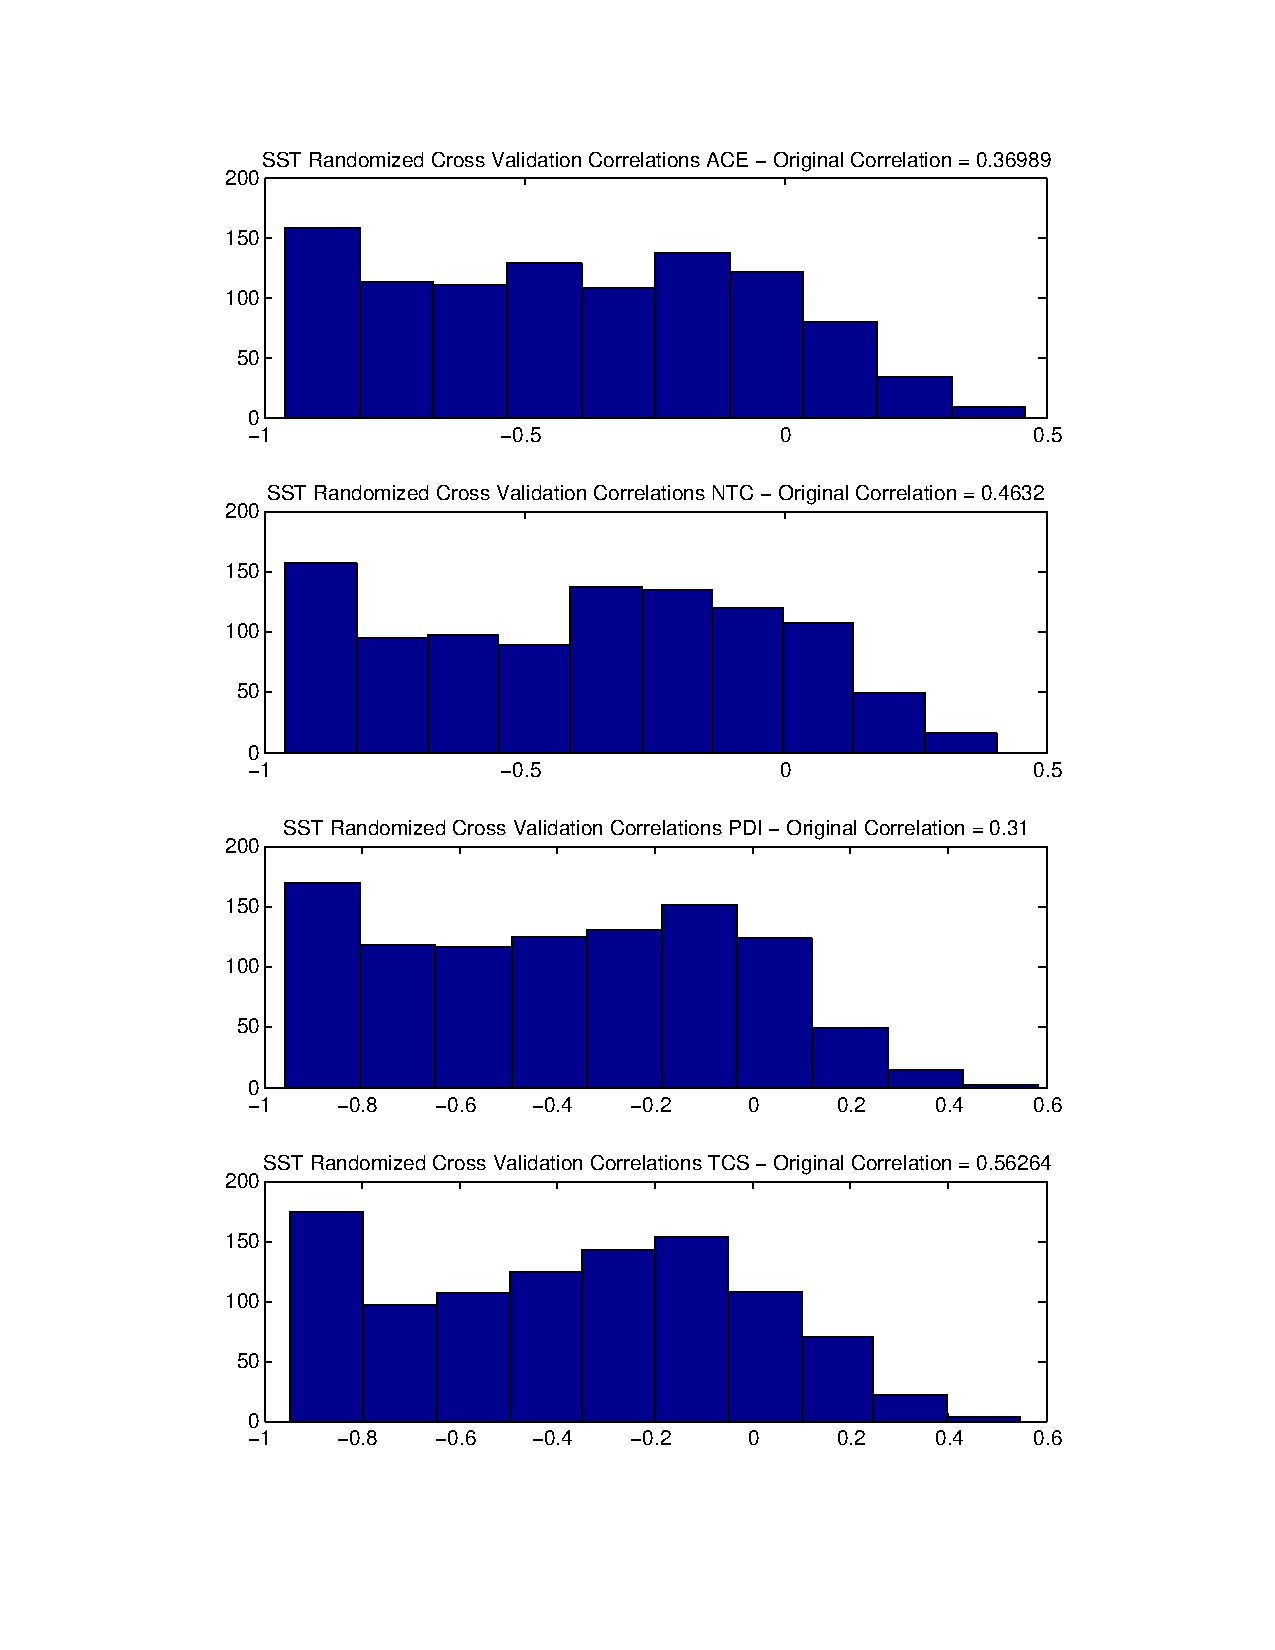
\includegraphics[ scale=0.7]{images/randomizedCrossValidationSST.pdf}
\subsection{Spatial SST + OLR Index}
For this index, we get two separate indices, one where we find the warmest SST box and one where we find the box with the highest OLR.  We then use both indices for the cross validation \newline
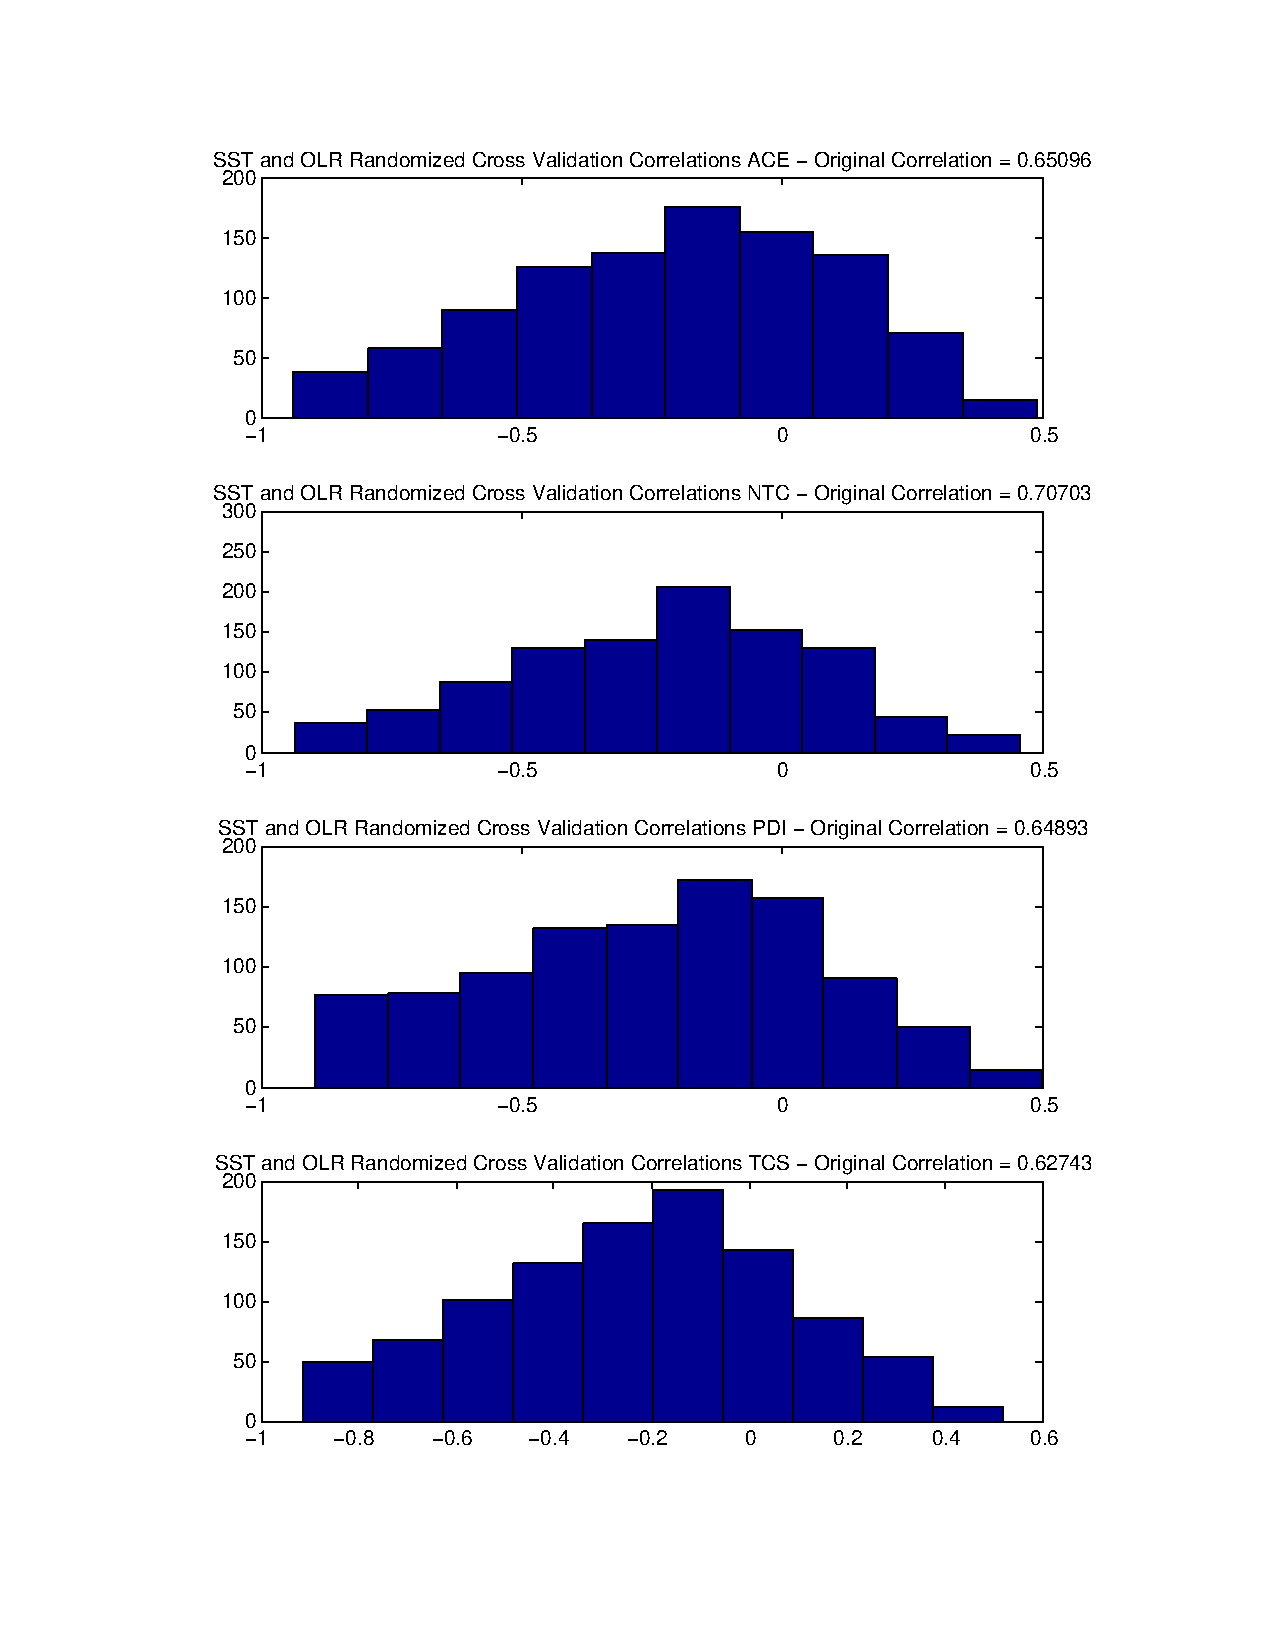
\includegraphics [scale = 0.6]{images/randomizedCrossValidationSSTAndOLR.pdf}
\newpage
\section{Varying Months Results}
This section contains the results where we vary the month range for which we average SST anomaly and NINO3.4 data for computing their respective indices.  For example, for month range 3-10, we average SST anomaly data from March - October for each year, and then look for the warmest box.  These results show the average of difference in composites, where we composite the highest years and the lowest years, take the difference of the two composites, and then average these differences within the main development region ($5^o$ to $20^o$ lat, $-70^o$ to $-15^o$ lon)

\subsection{Difference in Geopotential Height (1000-500 mbar)}
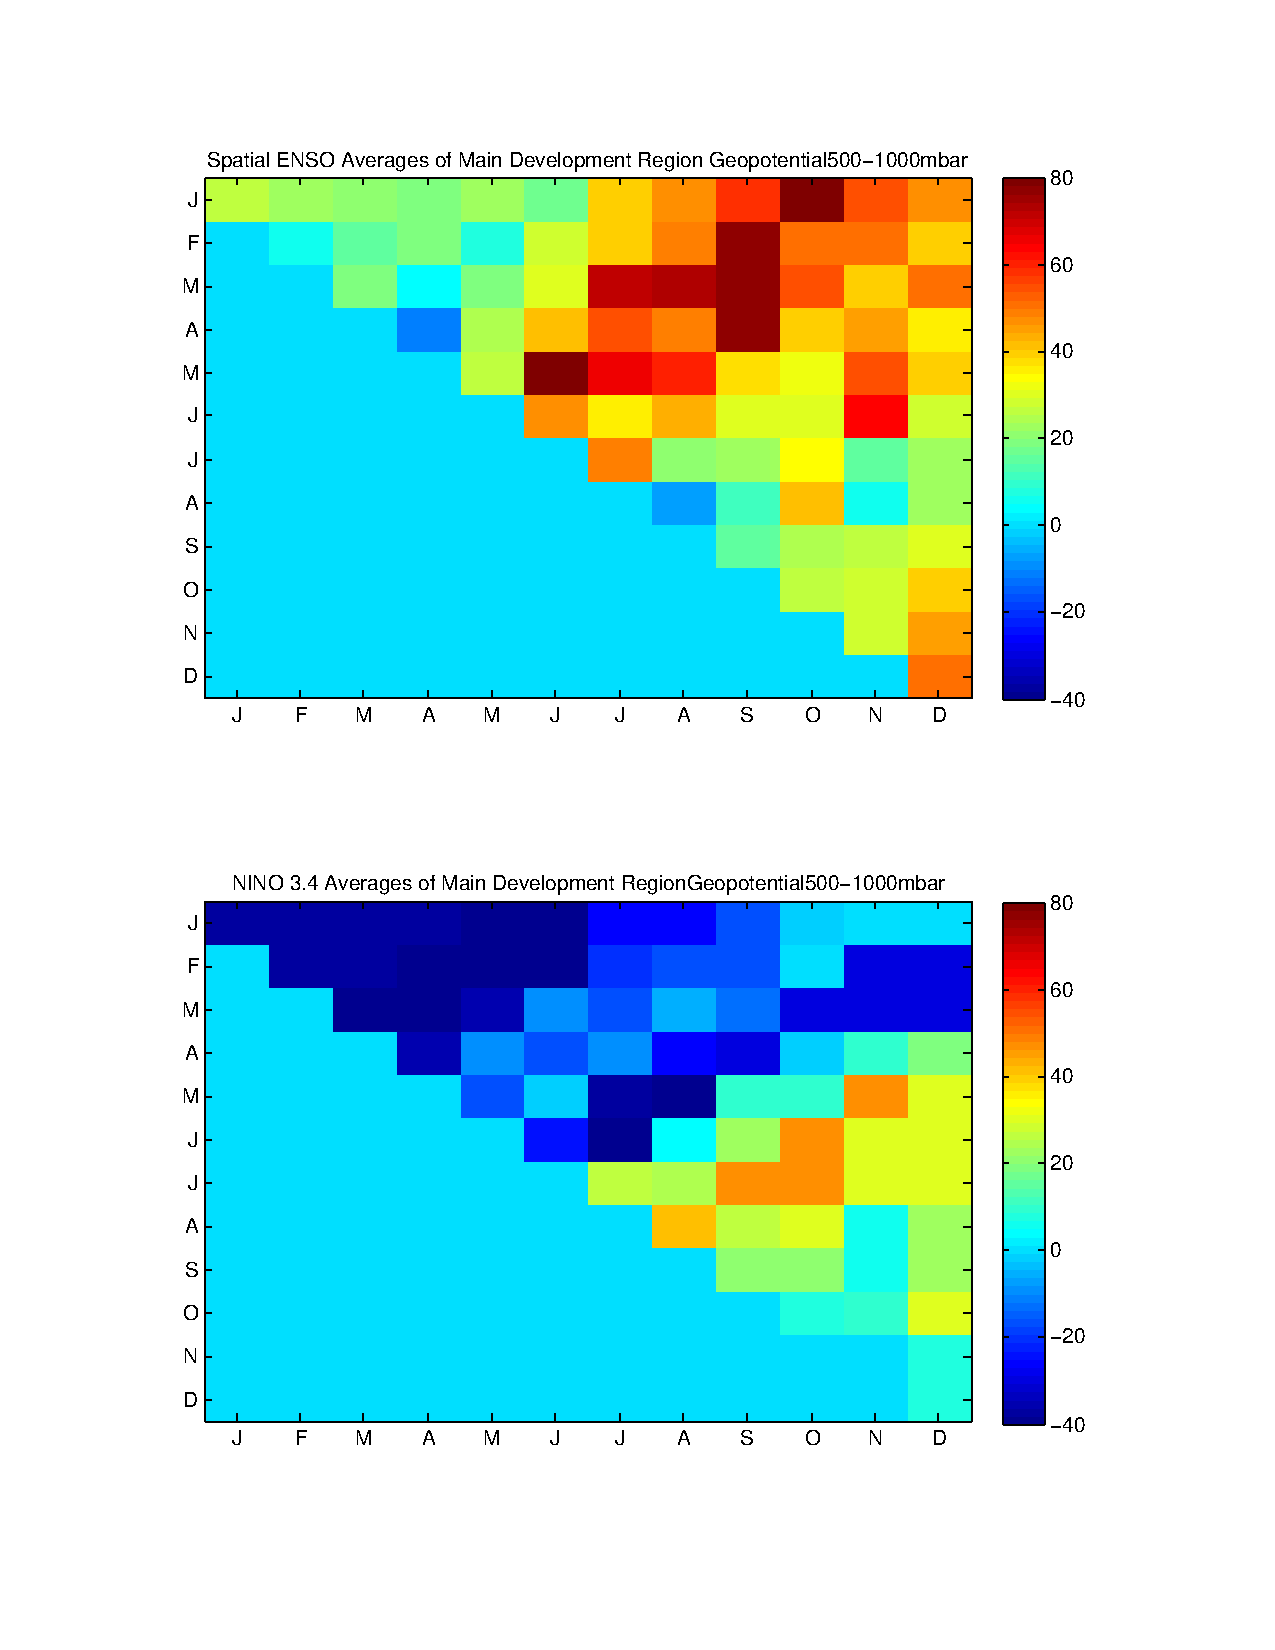
\includegraphics[scale=0.53]{images/varyingMonthsForMDRAveragesGeopotential500-1000mbar.pdf}

\subsection{Geopotential Height (500 mbar)}
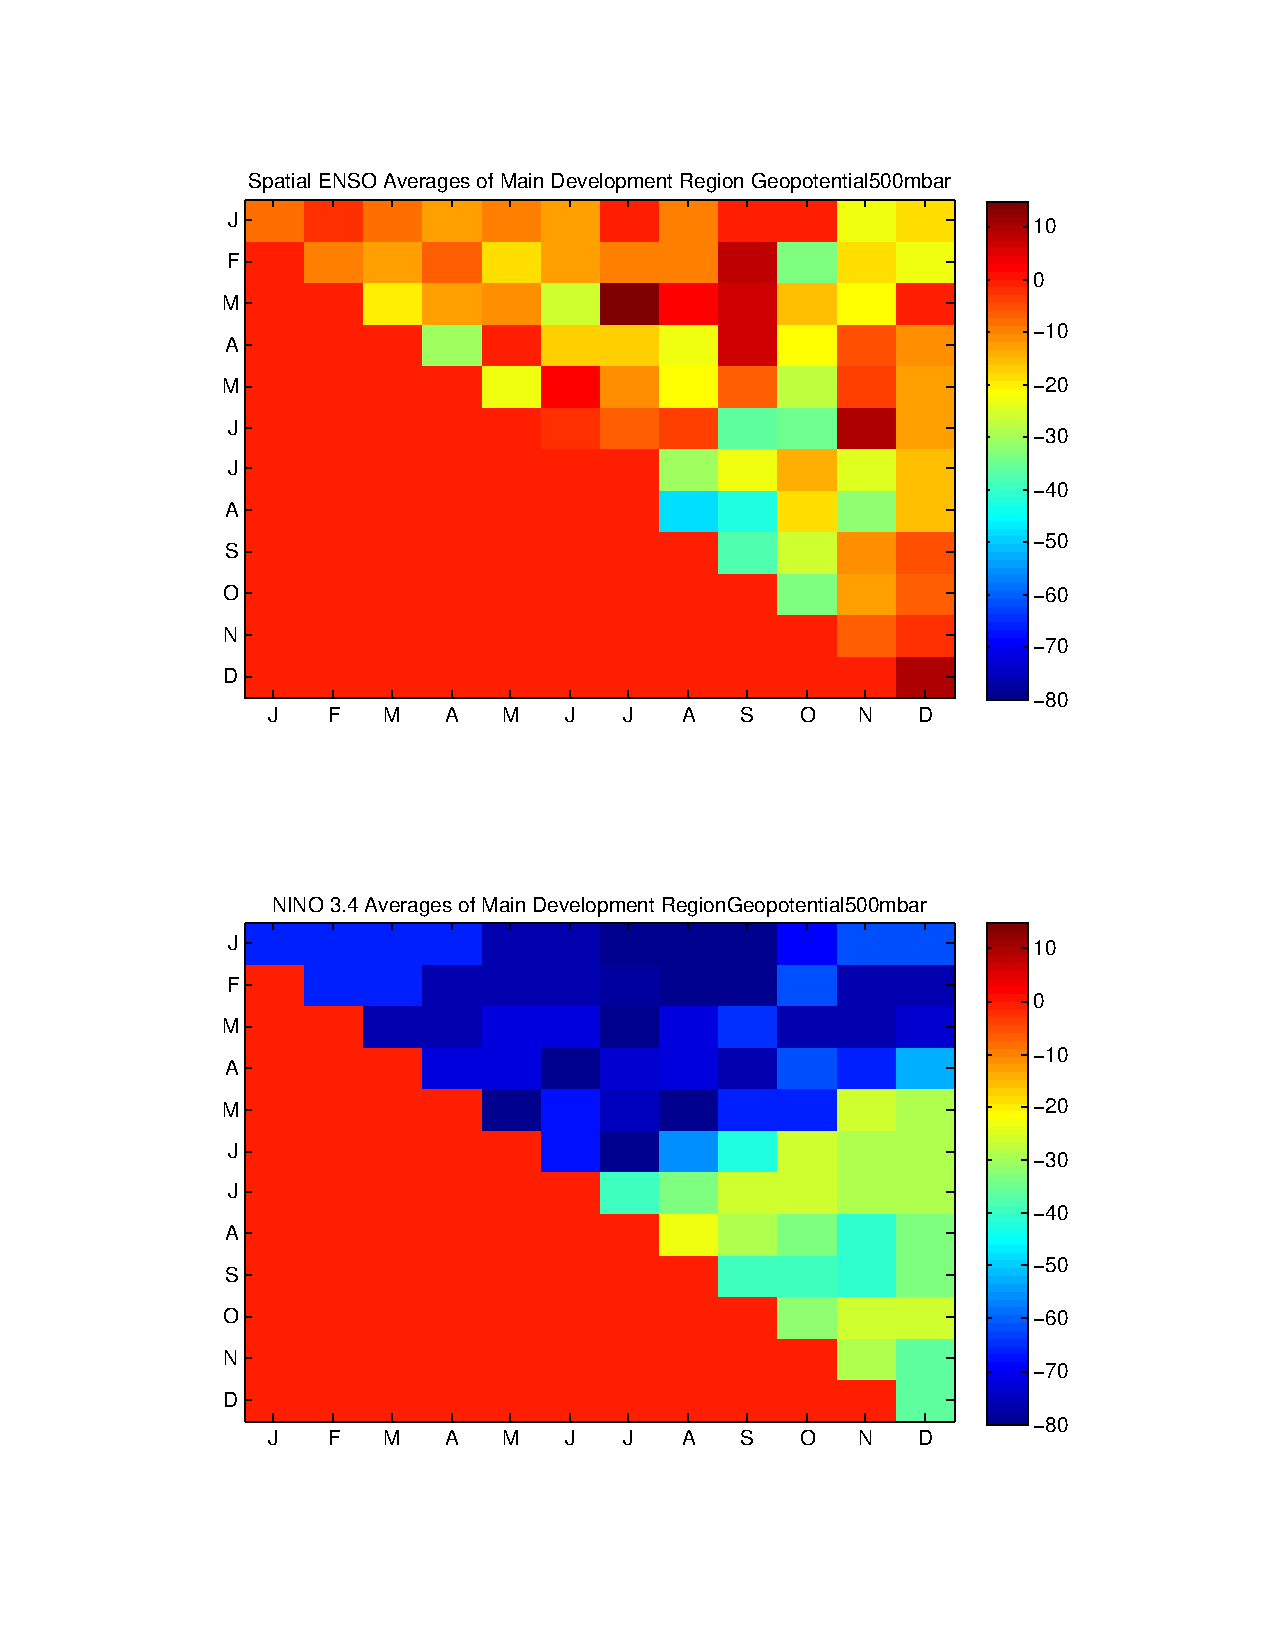
\includegraphics[scale=0.7]{images/varyingMonthsForMDRAveragesGeopotential500mbar.pdf}

\subsection{Sea Surface Temperature}
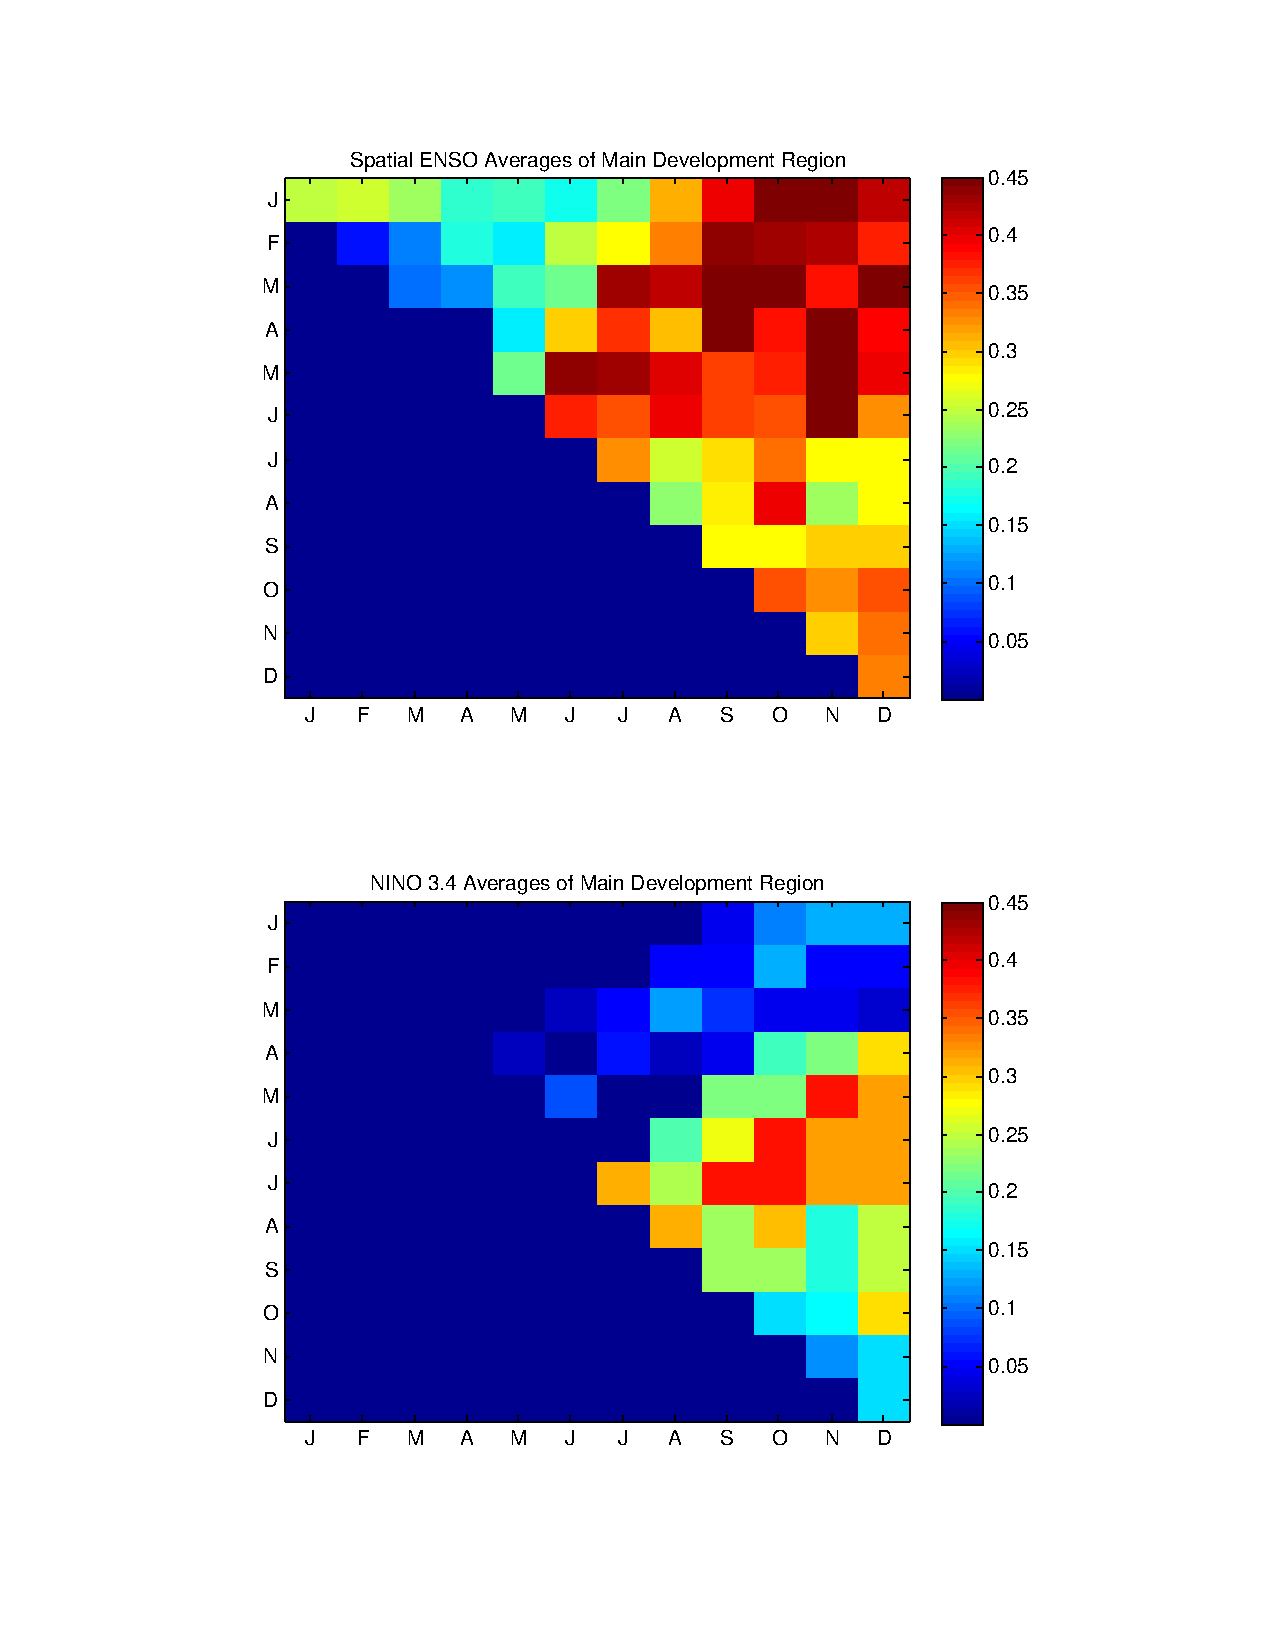
\includegraphics[scale=0.69]{images/varyingMonthsForMDRAveragesSST.pdf}

\subsection{Sea Level Pressure}
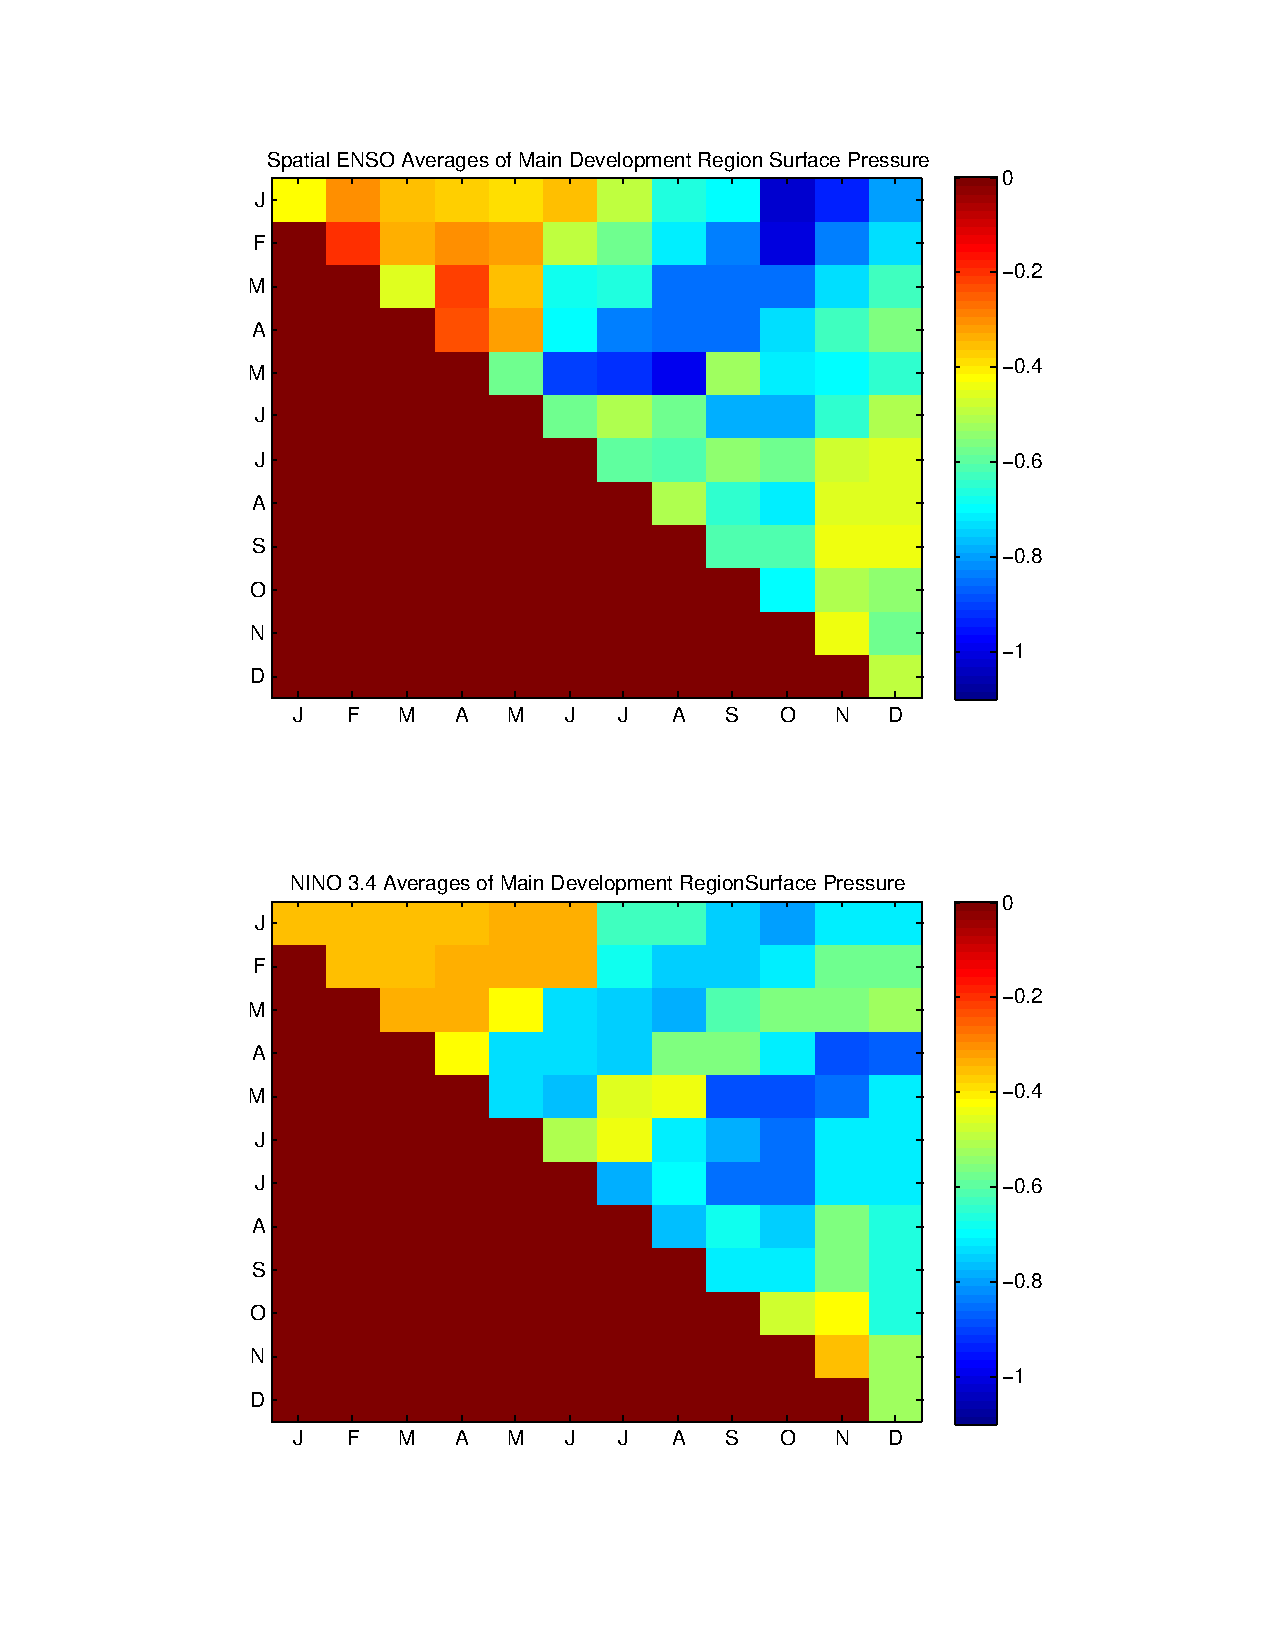
\includegraphics[scale=0.7]{images/varyingMonthsForMDRAveragesSurfacePressure.pdf}

\subsection{Wind Shear Between 850-200 mbar}
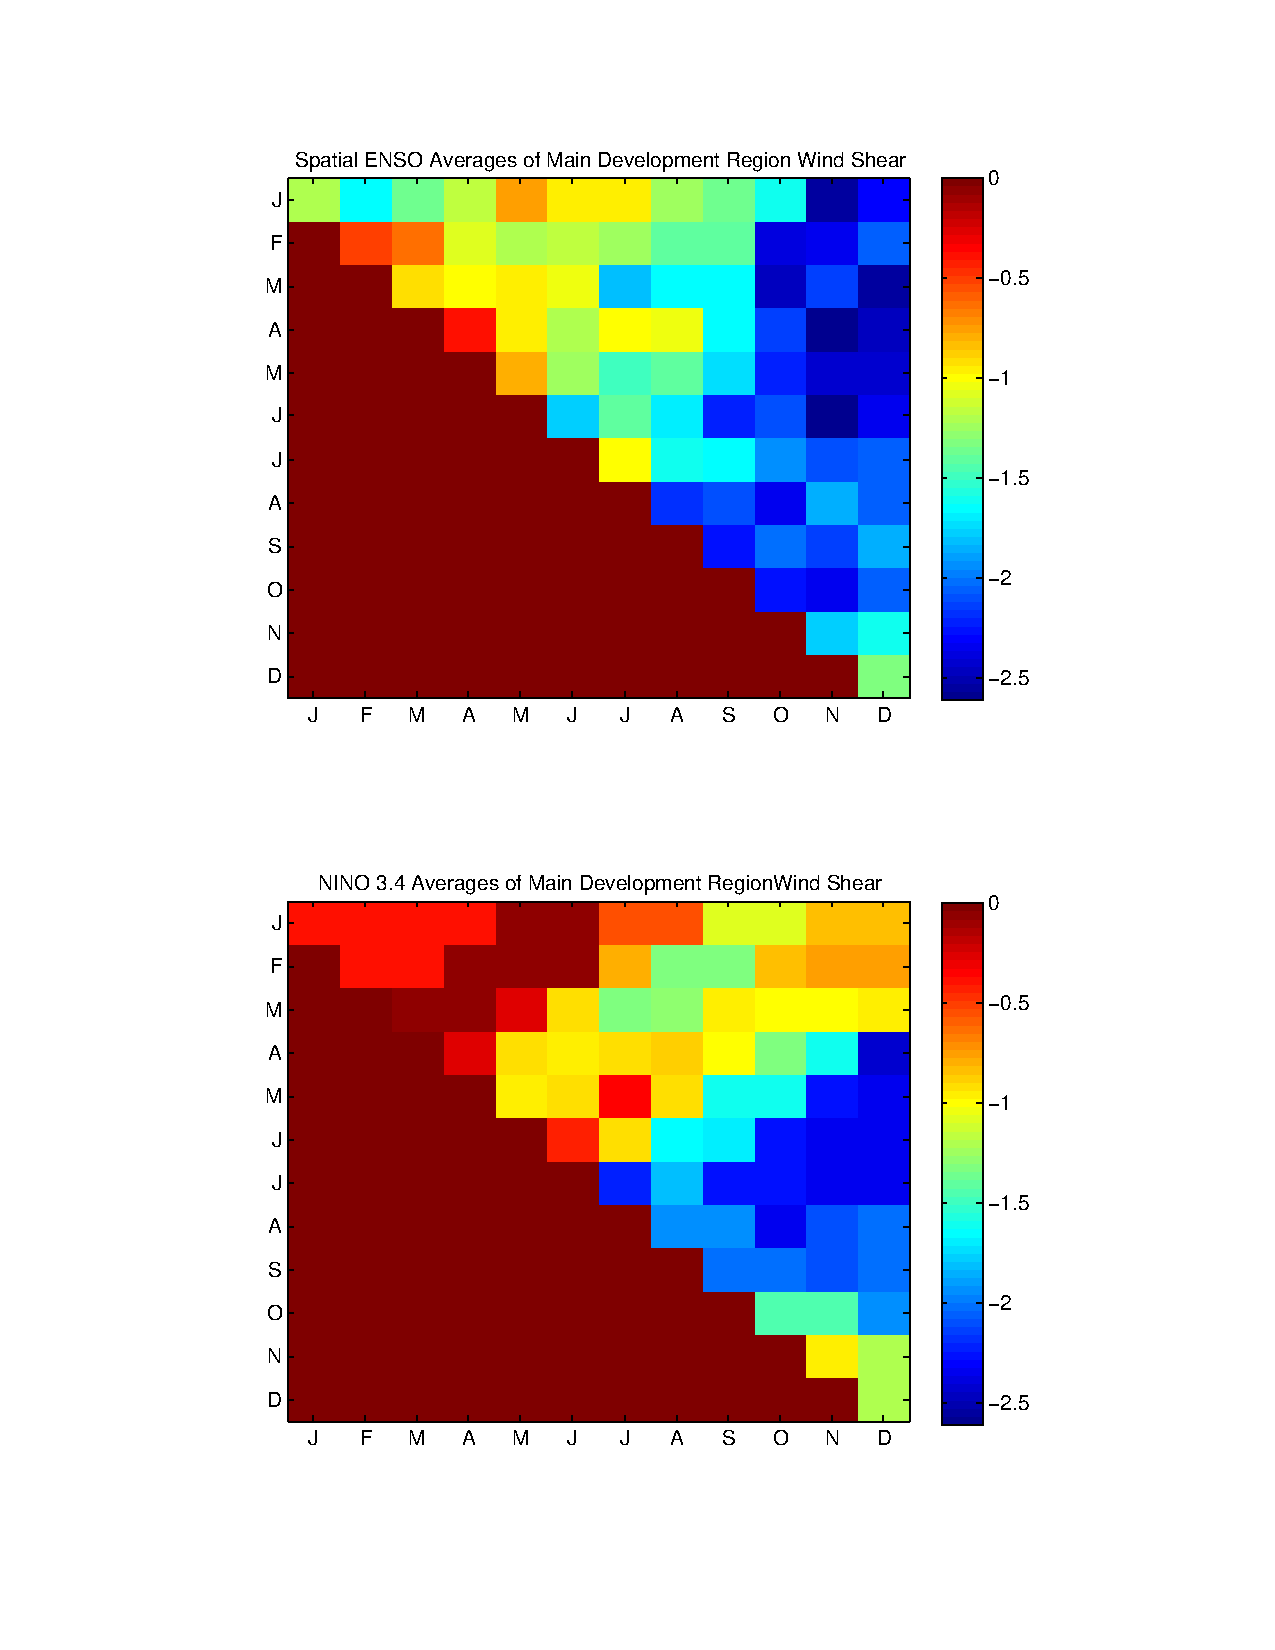
\includegraphics[scale=0.7]{images/varyingMonthsForMDRAveragesWindShear.pdf}

\section{Varying Standard Deviation Results}
This section contains the results where we vary the standard deviation threshold for which we pick the high and low years.  For example, if the standard deviation is 1, then the high years must be at least 1 standard deviation away from the mean, and the low years must be at least 1 standard deviation below the mean.  The y-axis of each graph shows the main development region average of the difference in composites.

\subsection{Difference in Geopotential Height (500-1000 mbar)}
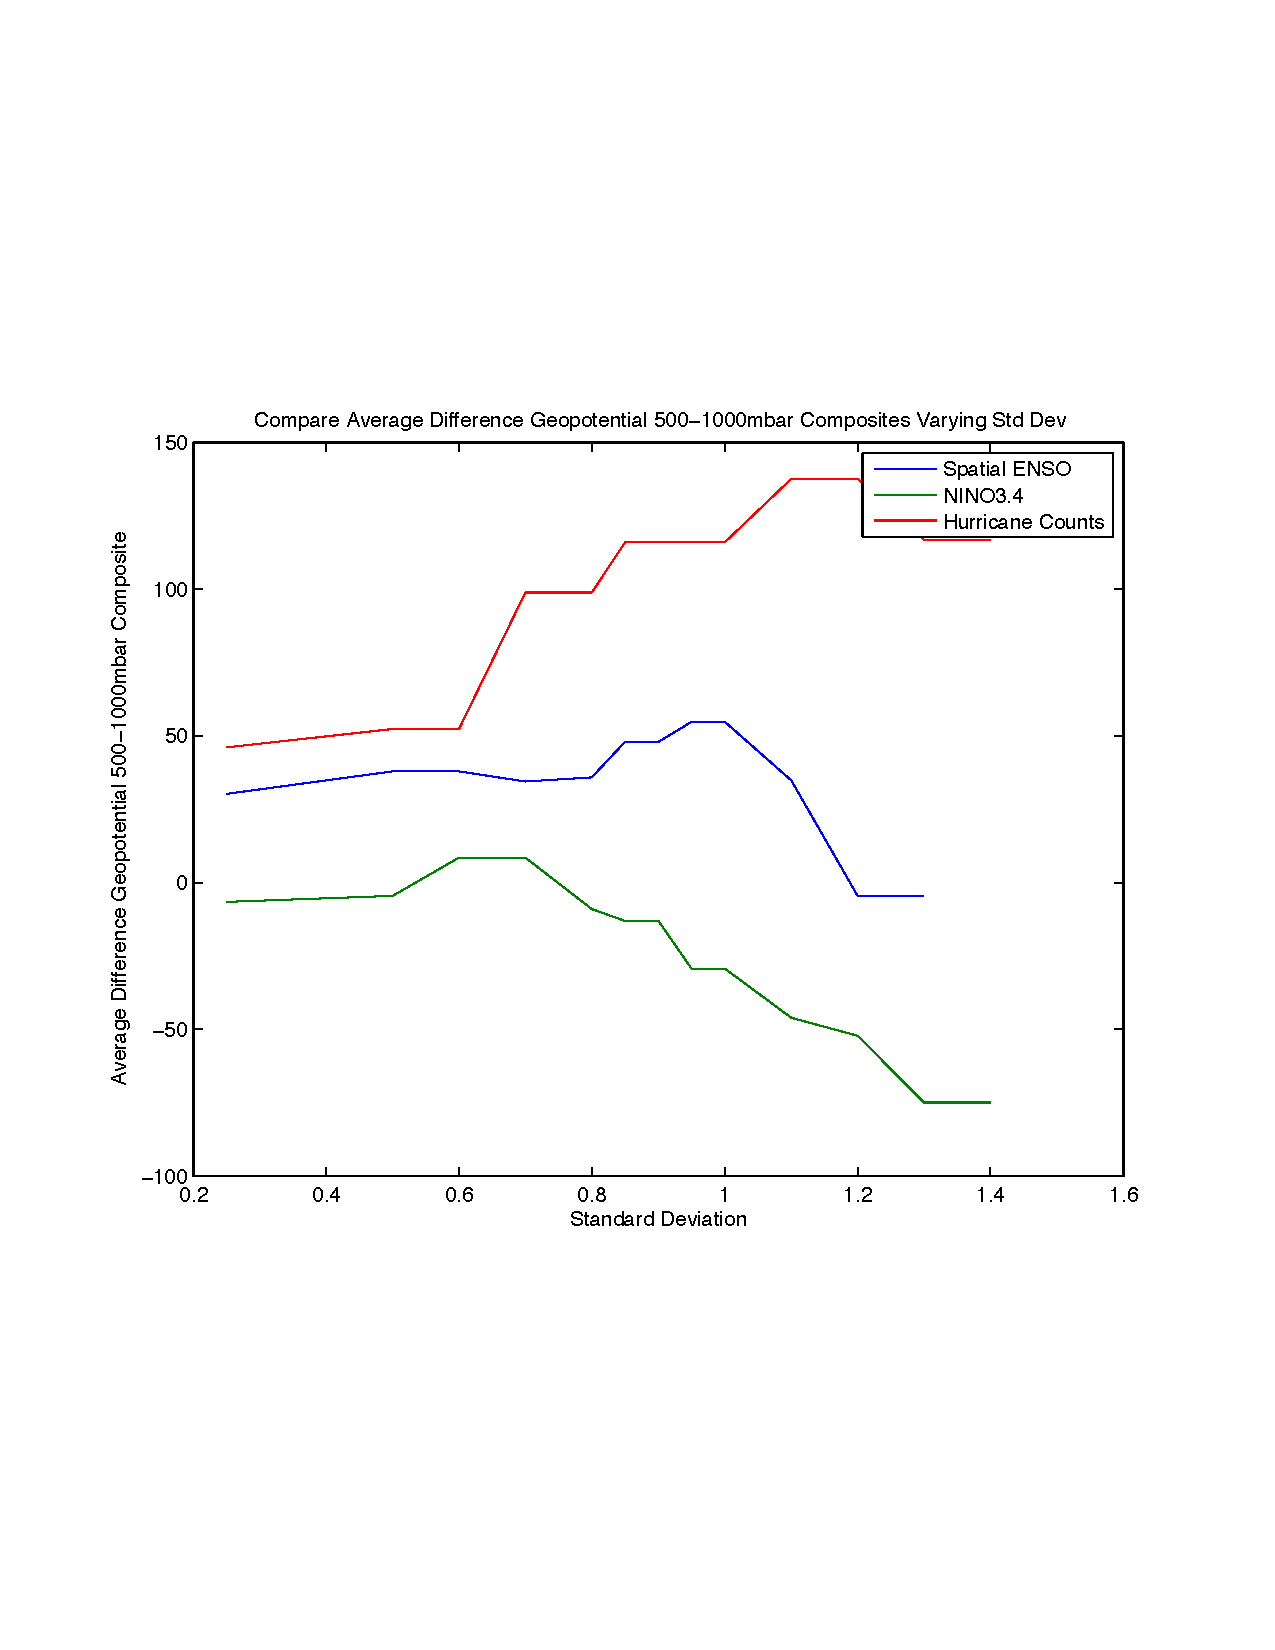
\includegraphics[scale = 0.6]{images/varyingStdDevForCompositesGeopotential500-1000mbar.pdf}

\newpage

\subsection{Geopotential Height (500 mbar)}
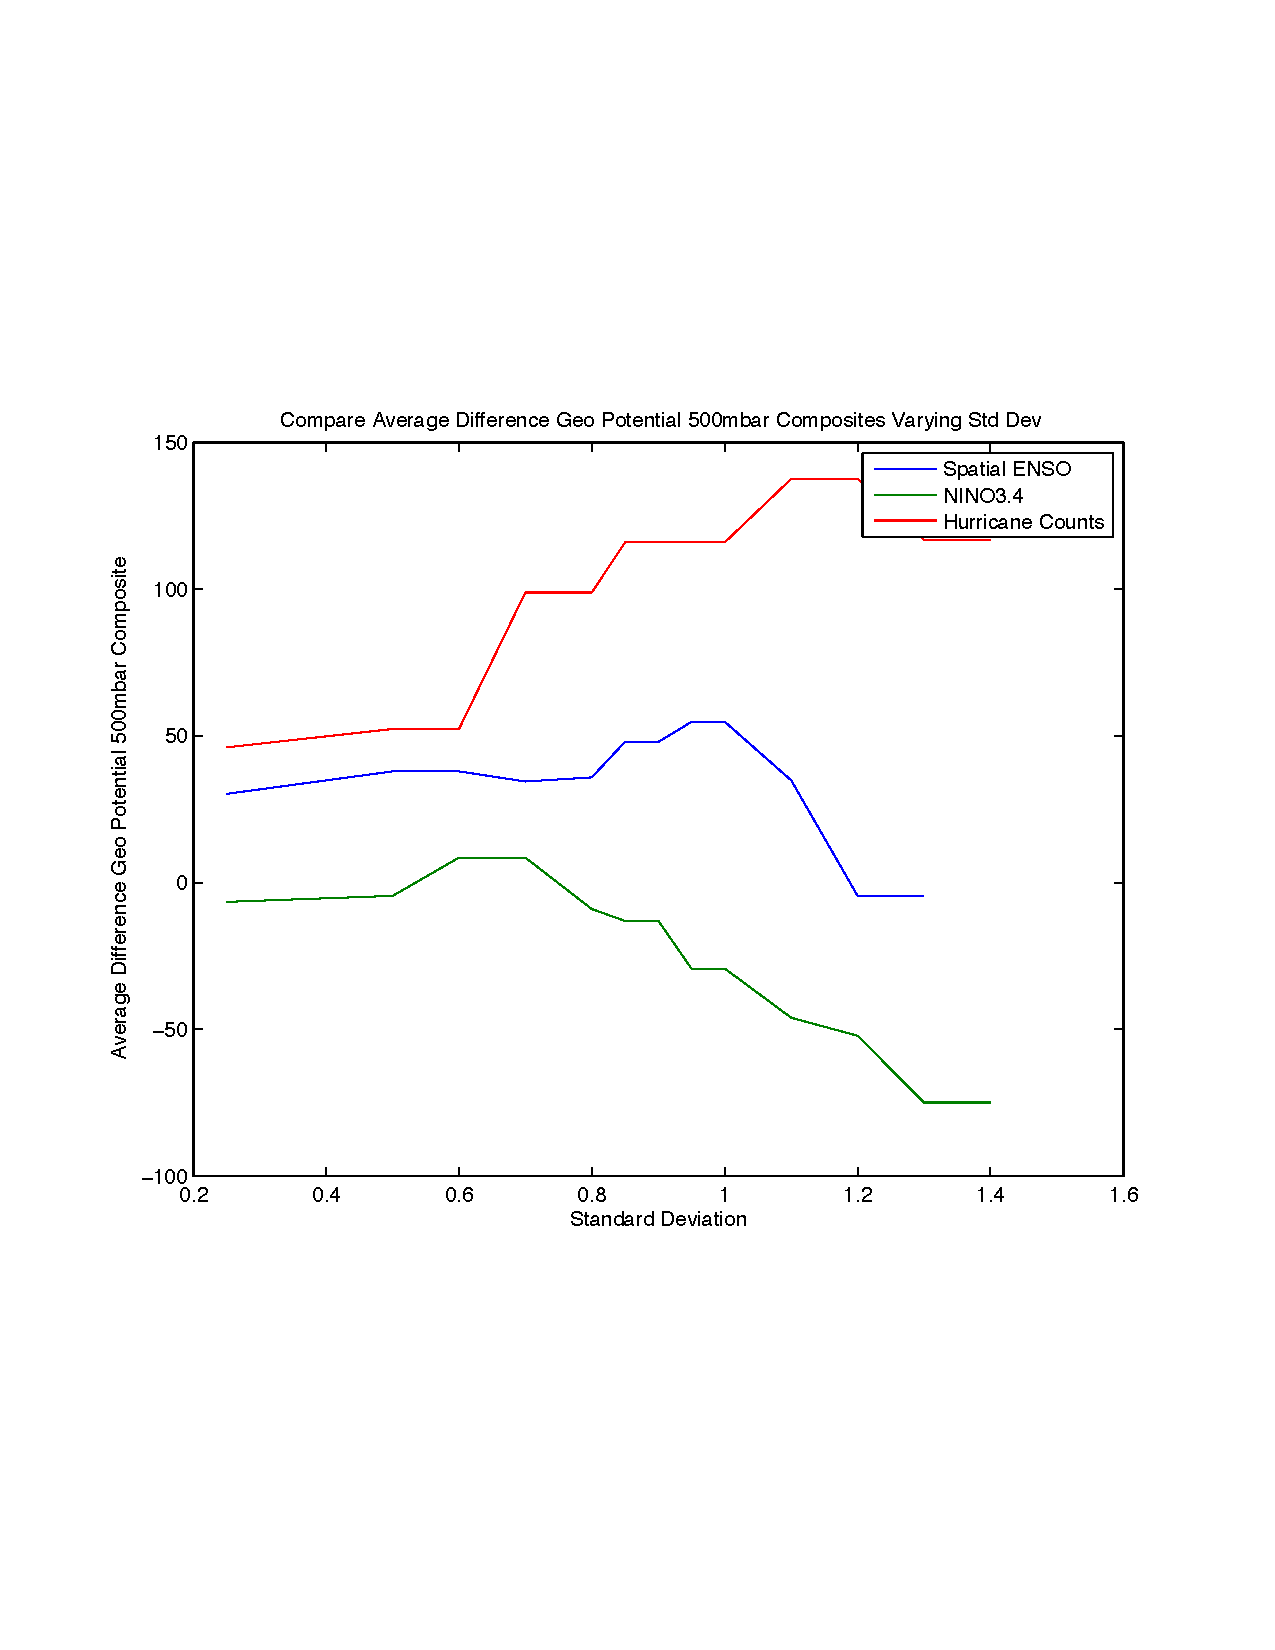
\includegraphics[scale=0.6]{images/varyingStdDevForCompositesGeopotential500mbar.pdf}

\subsection{Sea Surface Temperature}
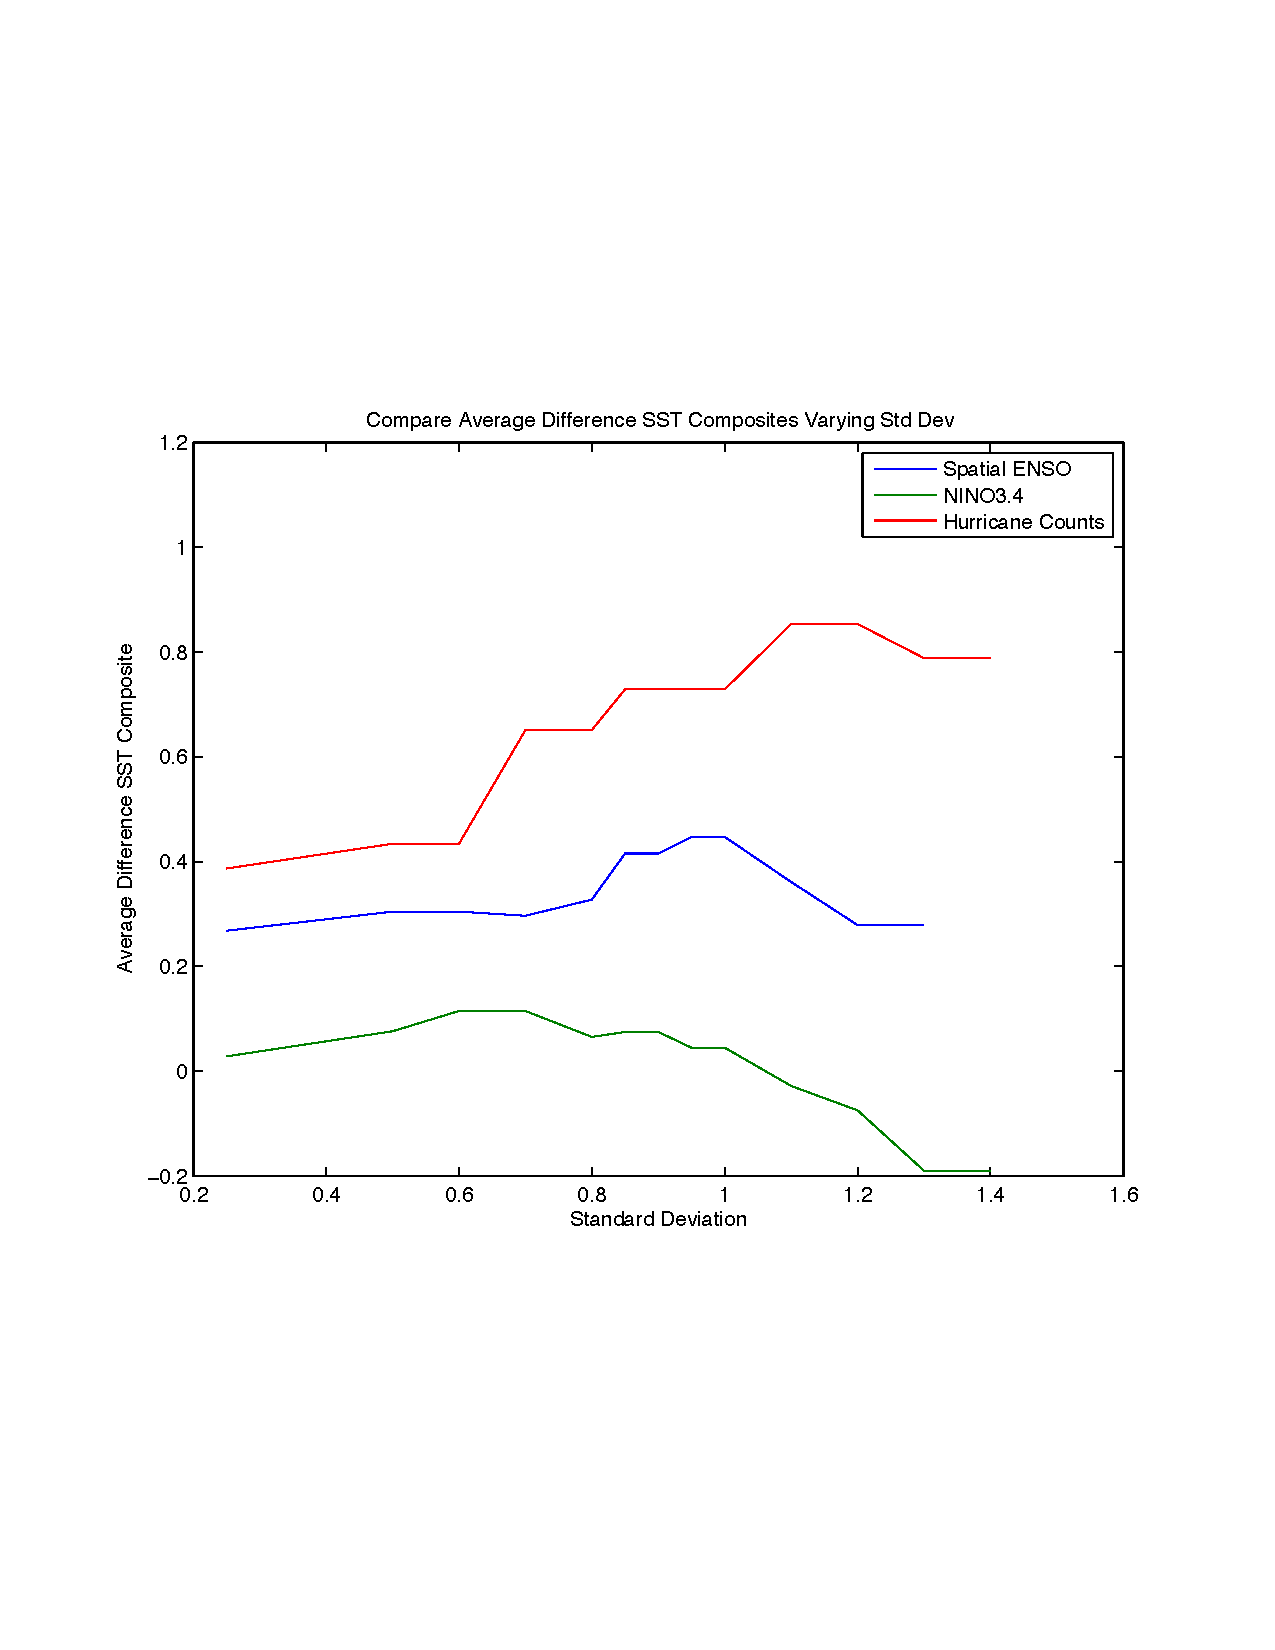
\includegraphics[scale = 0.6]{images/varyingStdDevForCompositesSST.pdf}

\subsection{Sea Level Pressure}
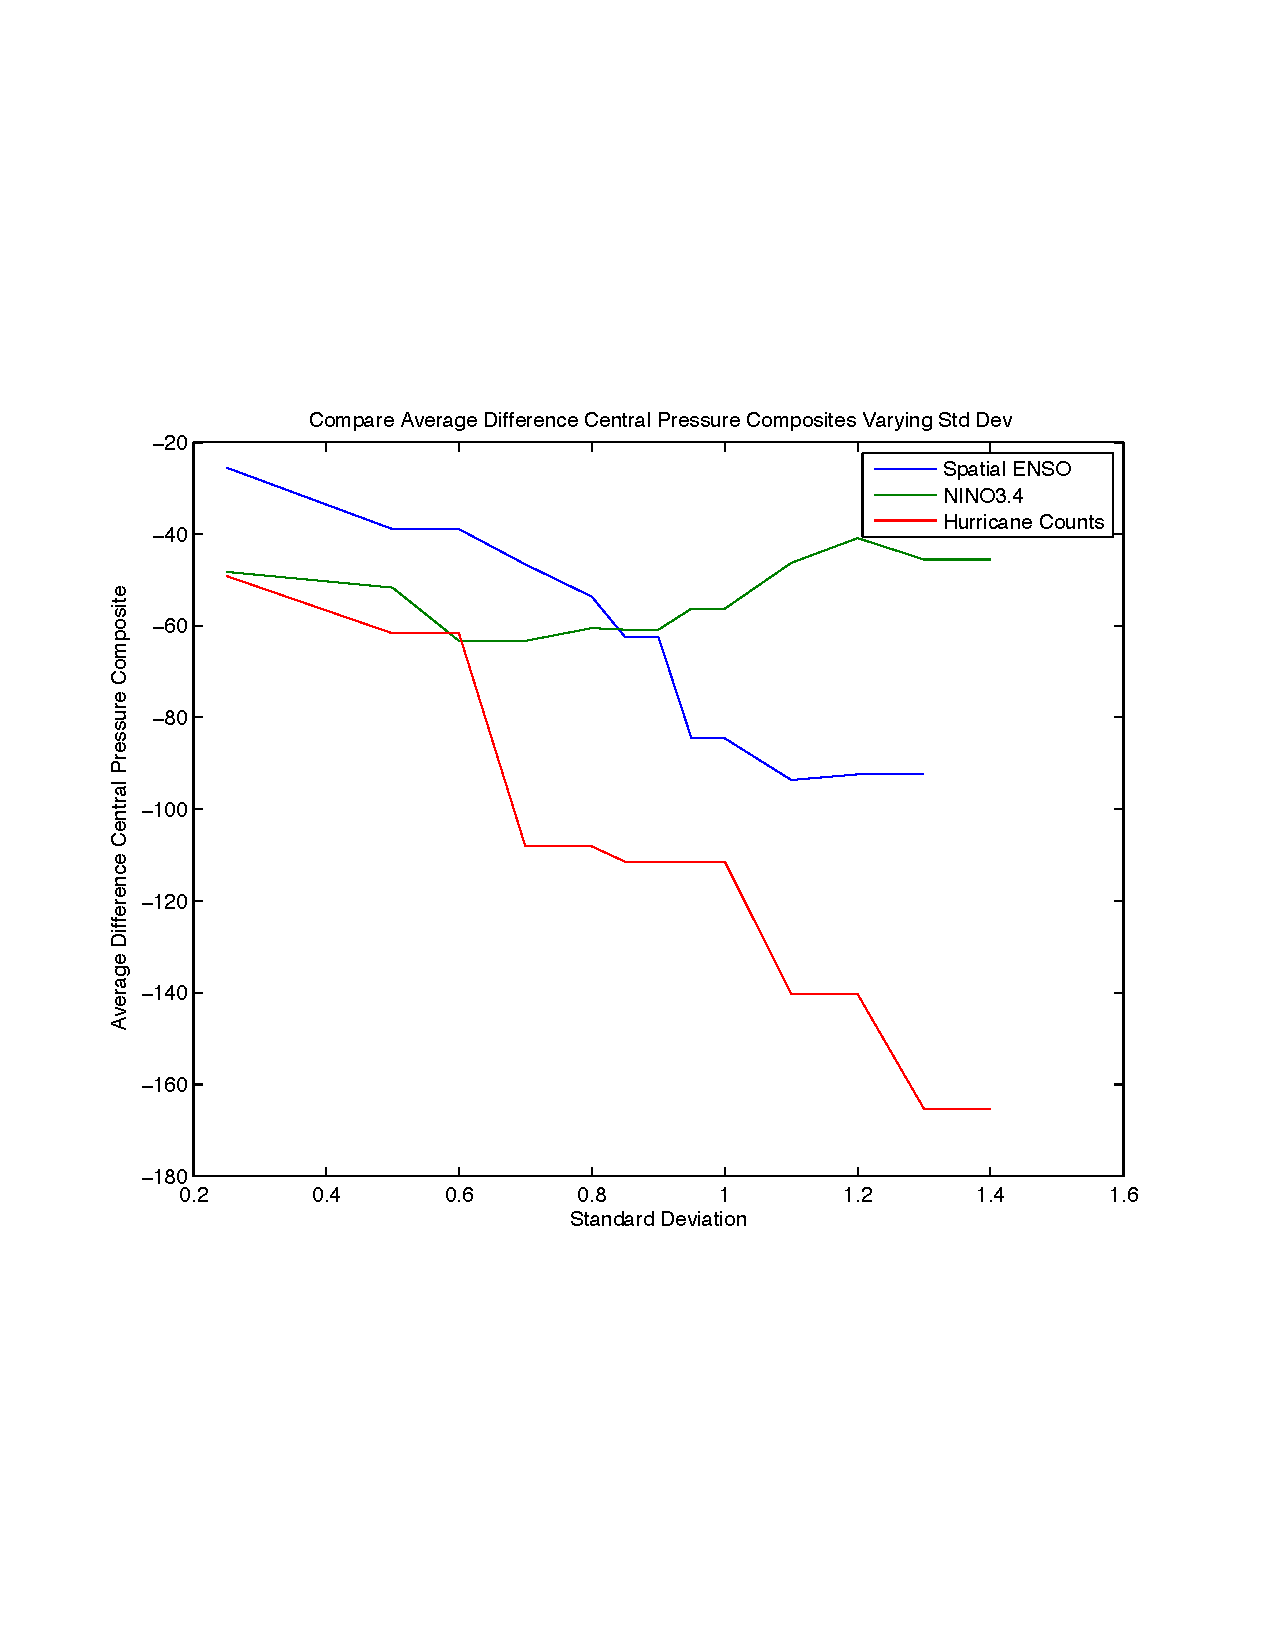
\includegraphics[scale = 0.6]{images/varyingStdDevForCompositesCentralPressure.pdf}

\subsection{Wind Shear Between 850-200 mbar}
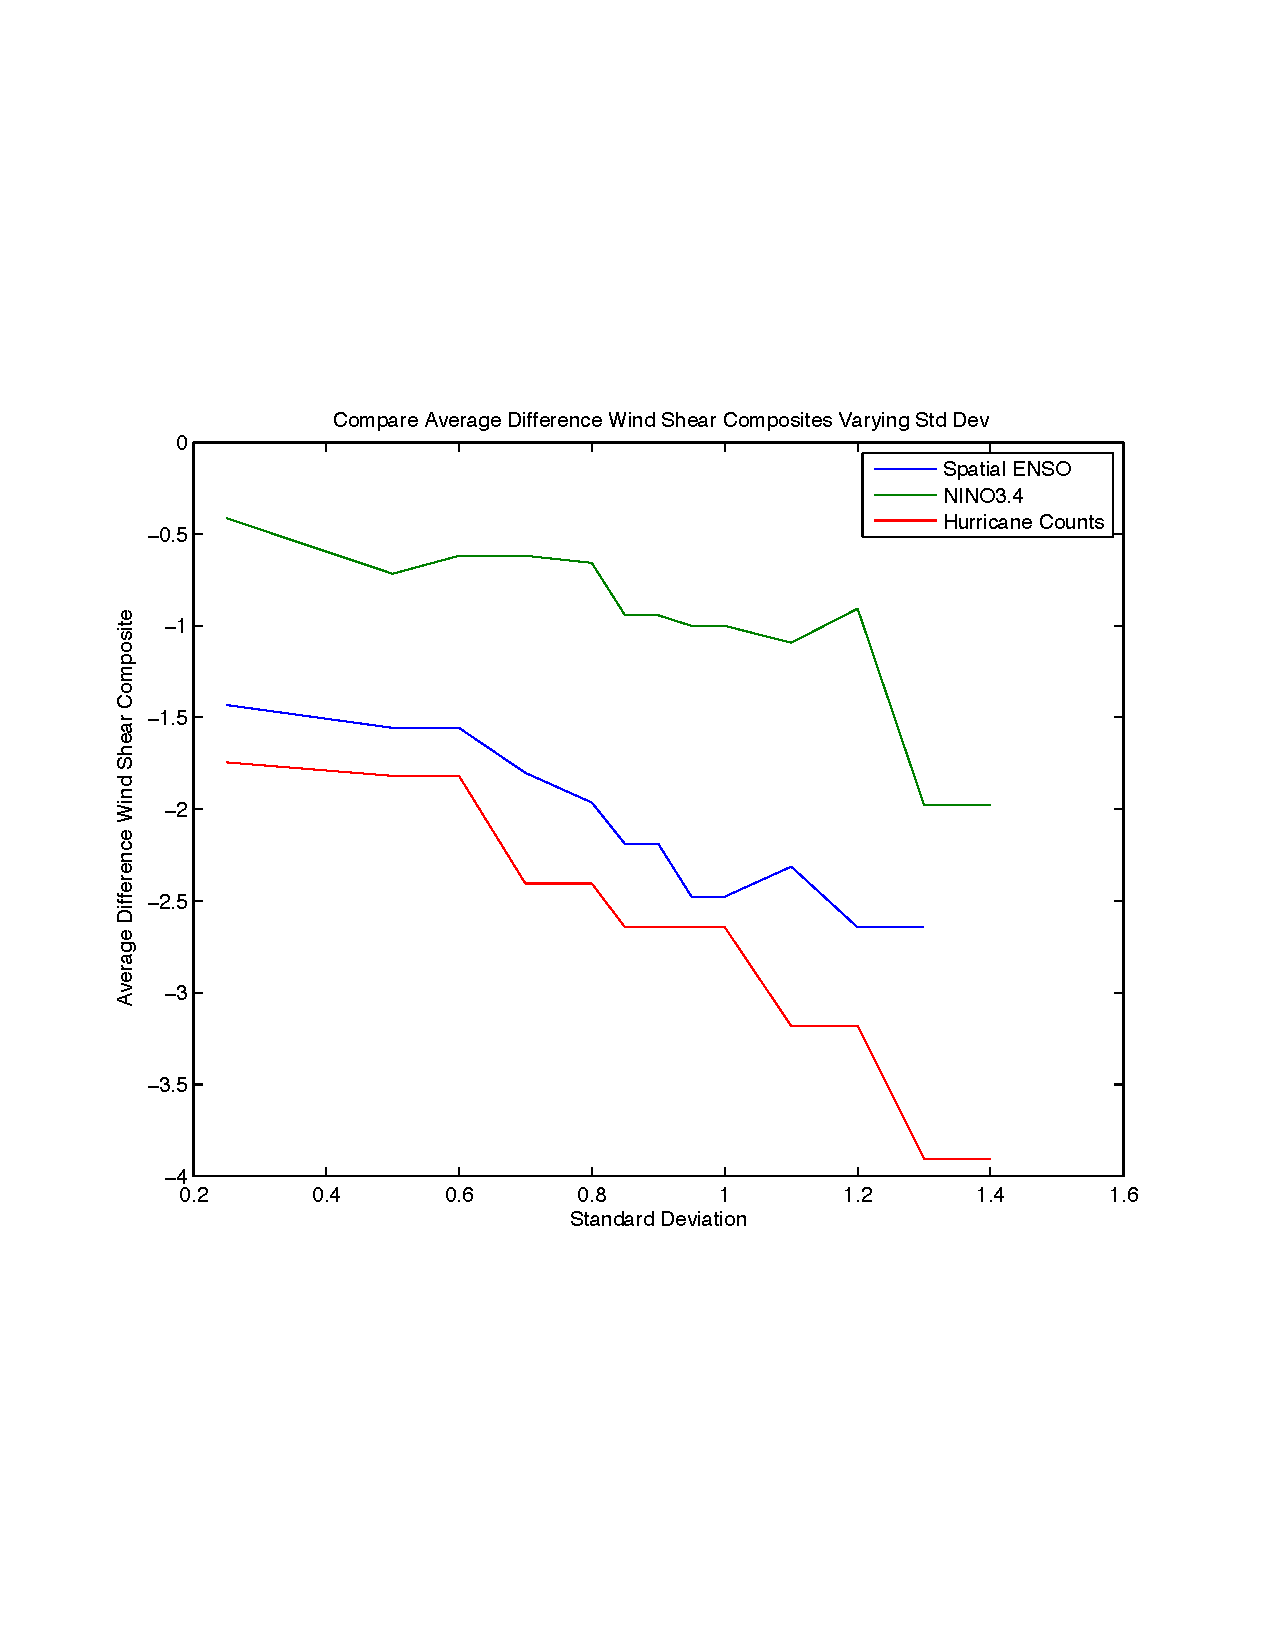
\includegraphics[scale=.6]{images/varyingStdDevForCompositesWindShear.pdf}

\section{Composite Results}
\subsection{Sea Surface Temperature}
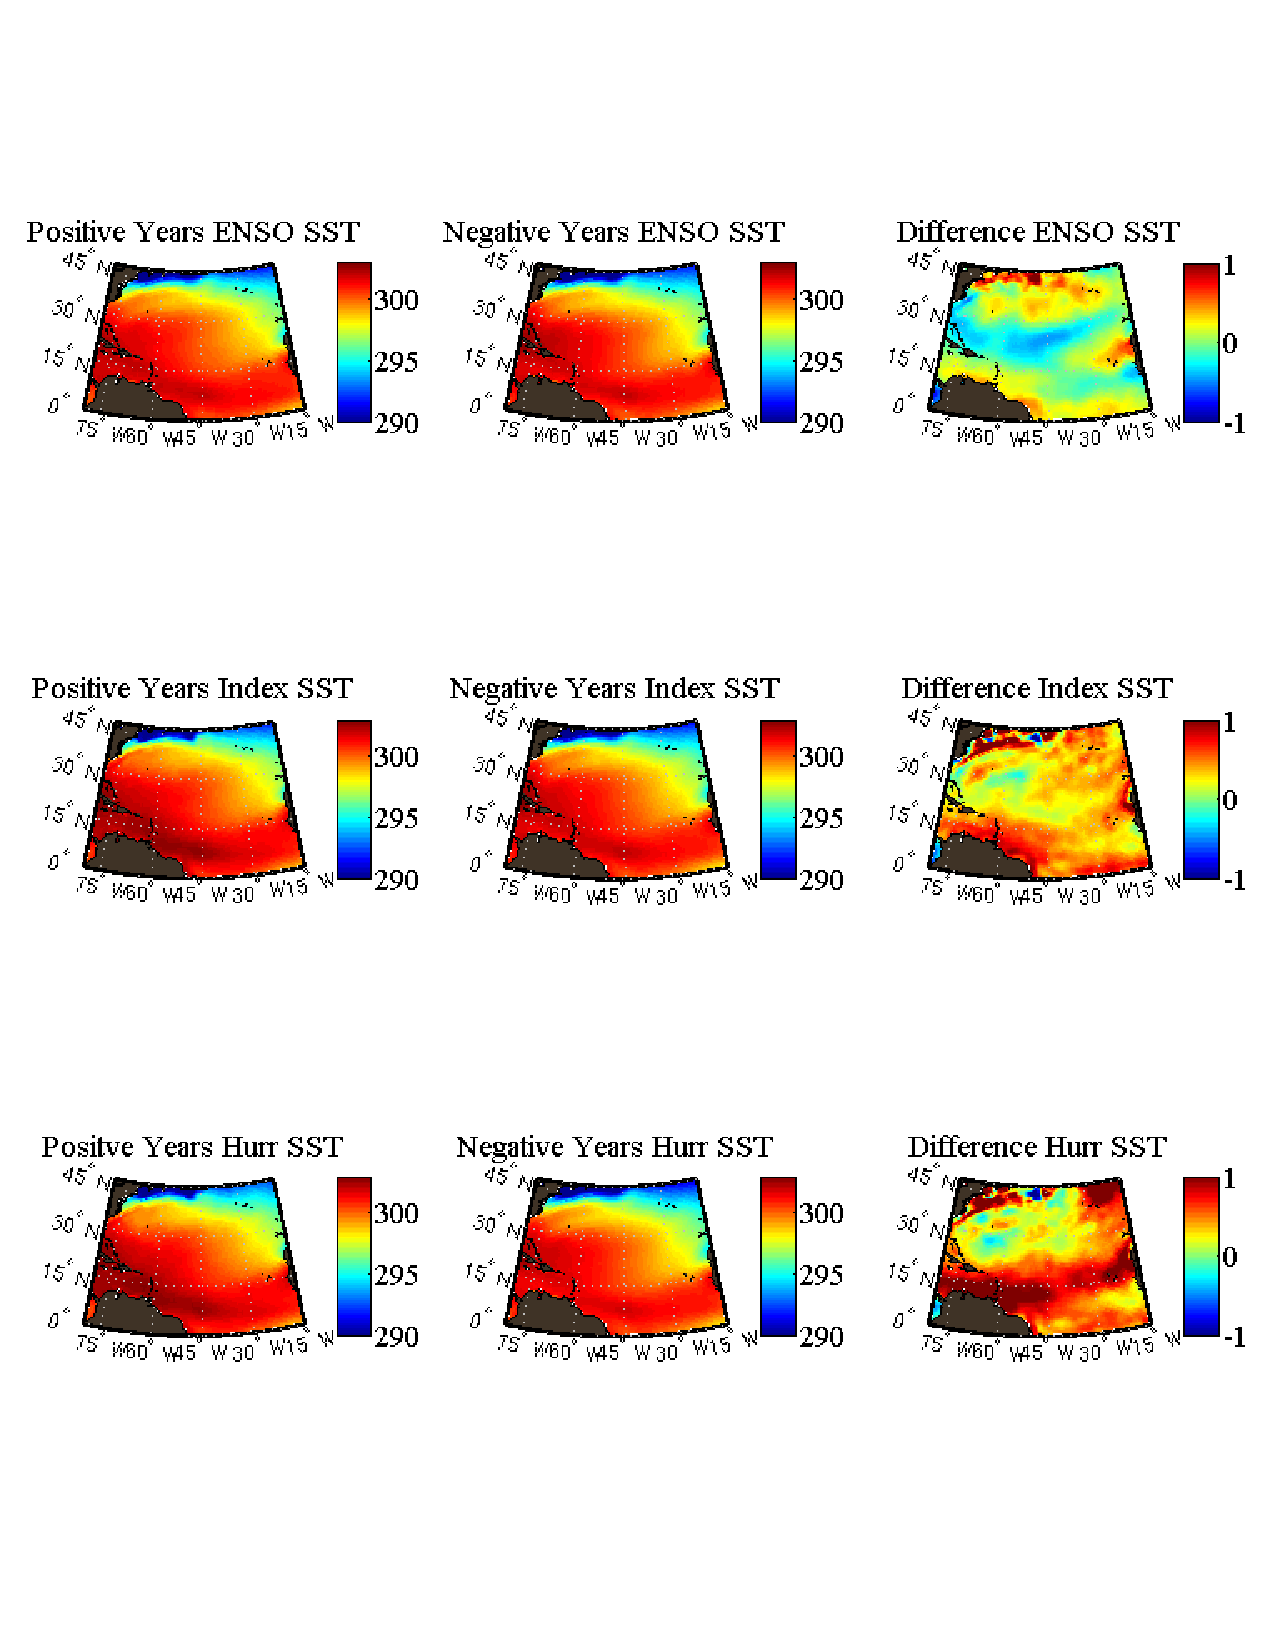
\includegraphics[scale=.75]{images/compareSSTComposites.pdf}
\newpage

\subsection{Wind Shear}
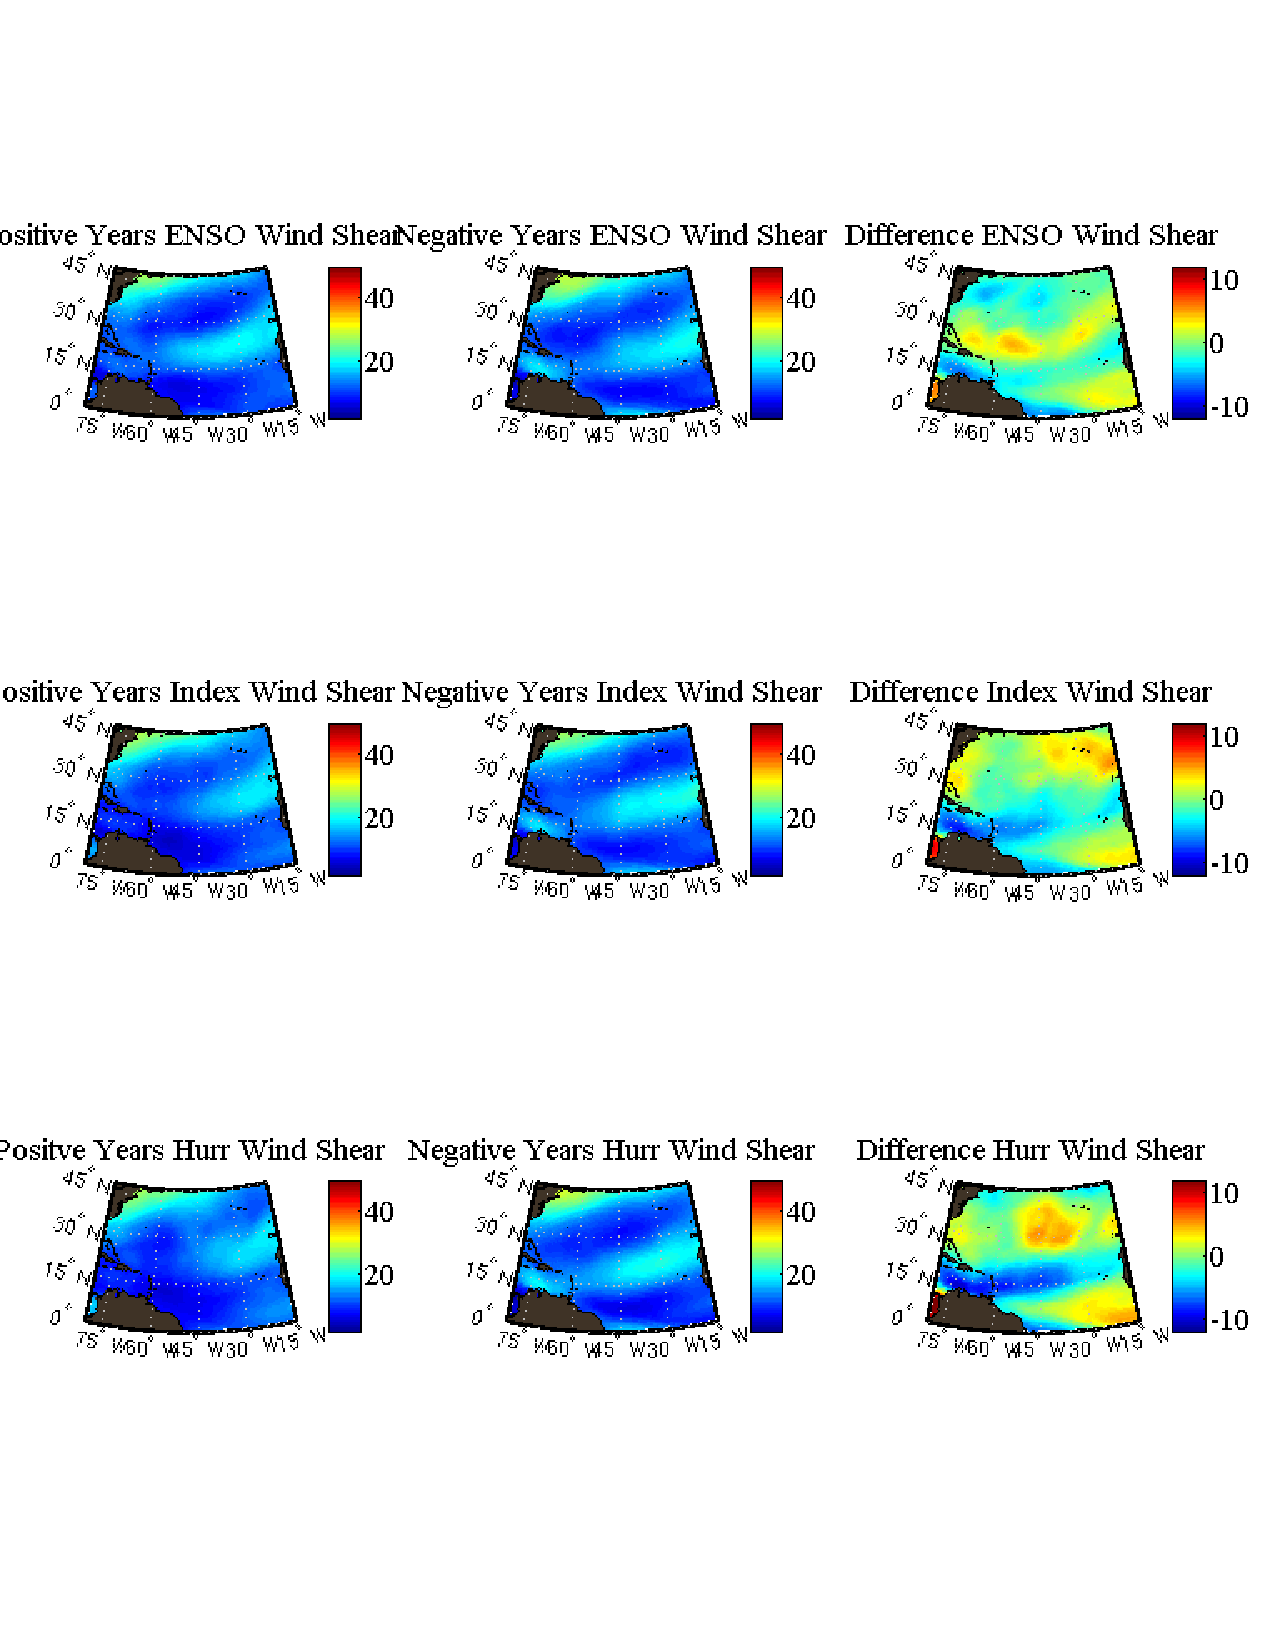
\includegraphics[scale=.75]{images/compareWindShearComposites.pdf}
\end{document}


















